
\documentclass[]{report}
\voffset=-1.5cm
\oddsidemargin=0.0cm
\textwidth = 480pt


\usepackage{amsmath}
\usepackage{graphicx}
\usepackage{amssymb}
\usepackage{framed}
\usepackage{multicol}
%\usepackage[paperwidth=21cm, paperheight=29.8cm]{geometry}
%\usepackage[angle=0,scale=1,color=black,hshift=-0.4cm,vshift=15cm]{background}
%\usepackage{multirow}
\usepackage{enumerate}

\usepackage{amsmath,amsfonts,amssymb}
\usepackage{color}
\usepackage{multirow}
\usepackage{eurosym}
\usepackage{framed}

%\input def.tex
%\input dsdef.tex
%\input rgb.tex

%\newcommand \la{\lambda}
%\newcommand \al{a}
%\newcommand \be{b}
\newcommand \x{\overline{x}}
\newcommand \y{\overline{y}}

\begin{document}
\section{3.4 Concepts of Solutions to 2-Player Matrix Games -
Minimax Solutions}
The minimax strategy of a player is the strategy that maximises
his/her expected payoff under the assumption that the other player
aims to minimise this payoff.
The minimax payoff of a player is the maximum expected payoff
that he/she can guarantee him/hirself.
In zero-sum games such a concept seems very reasonable, since by
minimising the expected reward of the opponent, an individual
maximises his/her expected reward.
%% 1 / 61
\subsection{Minimax Solutions}
One way of finding a player’s minimax strategy is to use linear
programming.
Suppose players choose one of two actions. In this case you can
think of the strategy of a player as the probability of playing the
first action, i.e. choice from the interval [0, 1]. The simplest
method of solution is to use calculus.
Denote the reward of Player i when Player 1 uses strategy p and
Player 2 uses strategy q by Ri(p, q).
2 / 61
%=================================================%
\subsection{Minimax Solutions - Example 3.4.1}
Find the minimax strategies and payoffs in the following matrix
game
A B
A (5,3) (2,6)
B (3,2) (4,5)
3 / 61
%=================================================%
\subsection{Minimax Solutions - Example 3.4.1}
\begin{itemize}
	\item Suppose Player 1 takes action A with probability p and Player 2
	takes action A with probability q. The expected reward of Player 1
	is given by
	R1(p, q) = 5pq+2p(1−q)+3(1−p)q+4(1−p)(1−q) = 4pq−2p−q+4.
	\item Player 1 assumes that Player 2 will minimise her payoff. 
		\item In order to
	derive which strategy of Player 2 minimises Player 1’s payoff, we
	calculate ∂R1(p,q)
	∂q
	(i.e. the rate of change of Player 1’s expected
	payoff with respect to the strategy of Player 2).
	\[∂R1(p, q)
	∂q
	= 4p − 1.\]
	\item	In general, this derivative will be a linear function of p.
\end{itemize}

4 / 61
%============================================%
\subsection{Minimax Solutions - Example 3.4.1}
There are three possibilities
\begin{enumerate}
	\item  ∂R1(p,q)
	∂q > 0 for all p ∈ [0, 1]. In this case to minimise
	Player 1’s payoff, Player 2 should play q = 0 (i.e.
	always take his second action). The minimax strategy
	of Player 1 is to take the action that maximises her
	reward when Player 2 takes his second action.
	\item  ∂R1(p,q)
	∂q < 0 for all p ∈ [0, 1]. In this case to minimise
	Player 1’s payoff, Player 2 should play q = 1 (i.e.
	always take his first action). The minimax strategy of
	Player 1 is to take the action that maximises her
	reward when Player 2 takes his first action.
	\item There exists some p ∈ [0, 1] such that ∂R1(p,q)
	∂q = 0.
	When Player 1 uses this strategy, her expected payoff
	does not depend on the strategy used by Player 2.
	This is her minimax strategy.
\end{enumerate}

5 / 61
%=================================================%
\subsection{Minimax Solutions - Example 3.4.1}
∂R1(p, q)
∂q
= 0 ⇒ p =
1
4
.
We have
R1(
1
4
, q) = 4 − 2p = 3.5.
It follows that the minimax strategy of Player 1 is to choose action
A with probability 0.25. In this way she guarantees herself a payoff
of 3.5
%% 6 / 61
%=================================================%
\subsection{Minimax Solutions - Example 3.4.1}
It should be noted that if Player 1 chose p >
1
4
, then ∂R1(p,q)
∂q > 0
and Player 2 minimises Player 1’s reward by choosing q = 0, i.e.
Playing B.
In this case the payoff of Player 1 would be
R1(p, 0) = 4 − 2p < 3.5.
Similarly, if Player 1 chose p <
1
4
, then ∂R1(p,q)
∂q < 0 and Player 2
minimises Player 1’s reward by choosing q = 1, i.e. Playing A.
In this case the payoff of Player 1 would be
R1(p, 1) = 2p + 3 < 3.5. It is thus clear that 3.5 is the maximum
expected payoff that Player 1 can guarantee herself.
%% 7 / 61
%=================================================%
\subsection{Minimax Solutions - Example 3.4.1}
We can calculate the minimax strategy of Player 2 in an analogous
way, by deriving his expected payoff as a function of p and q and
differentiating with respect to p, the strategy of Player 1. We have
\[R2(p, q) = 3pq+6p(1−q)+2(1−p)q+5(1−p)(1−q) = p−3q+5.\]
Hence,
\[∂R2(p, q)
∂p
= 1 > 0.\]
It follows that Player 1 always minimises Player 2’s expected
reward by playing p = 0, i.e. always taking action B.
%% 8 / 61
%=================================================%
\subsection{Minimax Solutions - Example 3.4.1}
If Player 1 takes action B, then Player 2 should take action B.
This ensures him a payoff of 5.
Note: It can be seen from the payoff matrix that if Player 1’s aim
is to minimise Player 2’s payoff, then her action B dominates
action A.
This is due to the fact that Player 2’s reward is always smaller
when Player 1 plays B, whatever action Player 2 takes.
%% 9 / 61
%============================================%
\subsection{Minimax Solutions - Example 3.4.1}
Suppose both players use their minimax strategies, i.e. Player 1
chooses action A with probability 0.25 and Player 2 always chooses
action B.
The payoff of Player 1 is
\[R1(0.25A + 0.75B, B) = 0.25 × 2 + 0.75 × 4 = 3.5.\]
The payoff of Player 2 is
\[R2(0.25A + 0.75B, B) = 0.25 × 6 + 0.75 × 5 = 5.25,\] i.e. the
reward obtained by Player 2 is greater than his minimax payoff.
In general, if a player’s minimax strategy is a pure strategy, when
both players play their minimax strategies, he/she may obtain a
greater expected payoff than his/her minimax payoff.
%% 10 / 61
%===========================================%
\subsection{Concepts of Solutions to 2-Player Matrix Games - Pure
Nash equilibria}
A pair of actions (A
∗
, B
∗
) is a pure Nash equilibrium if
R1(A
∗
, B
∗
) ≥ R1(A, B
∗
); R2(A
∗
, B
∗
) ≥ R2(A
∗
, B).
for any action A available to Player 1 and any action B available
to Player 2.
That is to say that a pair of actions is a Nash equilibrium if neither
player can gain by unilaterally changing their action (i.e. changing
their action whilst the other player does not change their action).
The value of the game corresponding to an equilibrium is the
vector of expected payoffs obtained by the players.
%%- 11 / 61
%=================================%
\subsection{Concepts of Solutions to 2-Player Matrix Games - Strong
Nash equilibria}
A pair of actions (A
∗
, B
∗
) is a strong Nash equilibrium if
R1(A
∗
, B
∗
) > R1(A, B
∗
); R2(A
∗
, B
∗
) > R2(A
∗
, B).
for any action A 6= A
∗
available to Player 1 and any action B 6= B
∗
available to Player 2.
i.e. a pair of actions is a strong Nash equilibrium if both players
would lose by unilaterally changing their action.
Any Nash equilibrium that is not strong is called weak.
%% 12 / 61
%================================%
\subsection{Concepts of Solutions to 2-Player Matrix Games - Mixed
Nash equilibria}
A pair of mixed strategies, denoted (M1, M2) is a mixed Nash
equilibrium if
\[R1(M1, M2) ≥ R1(A, M2); R2(M1, M2) ≥ R2(M1, B)\]
for any action (pure strategy) A available to Player 1 and any
action B available to Player 2.
\begin{itemize}
	\item It should be noted that the expected reward Player 1 obtains when
	he plays a mixed strategy M against M2 is a weighted average of
	the expected rewards of playing his pure actions against M2, where
	the weights correspond to the probability of playing each action.
	\item It follows that player 1 cannot do better against M2 than by using
	the best pure action against M2, i.e. if Player 1 cannot gain by
	switching to a pure strategy, then she cannot gain by switching to
	any mixed strategy.
\end{itemize}

%%- 13 / 61
%================================%
\subsection{The Bishop-Cannings Theorem}
\begin{itemize}
	\item The support of a mixed strategy M1 is the set of actions that are
	played with a positive probability under M1.
\item Suppose (M1, M2) is a Nash equilibrium pair of mixed strategies
	and the support of M1 is S. We have
	R1(A, M2) = R1(M1, M2), ∀A ∈ S; R1(B, M2) < R1(M1, M2), ∀B ∈/ S.
\item This is intuitively clear, since if a player uses actions A and B
	under a mixed strategy, then at equilibrium these actions must give
	the same expected reward, otherwise one action would be preferred
	over the other.
\item It follows that at such an equilibrium all actions in the support of
	M1 must give the same expected reward, which thus has to be
	equal to the expected reward of using M1 (which is calculated as a
	weighted average). Thus all mixed Nash equilibria are weak.
\end{itemize}

14 / 61
%================================%
\subsection{Nash Equilibria - Results}
Every matrix game has at least one Nash equilibrium.
If there is a unique pure Nash equilibrium of a 2 × 2 game (i.e. a
game in which both players have just 2 possible actions), then that
is the only Nash equilibrium.
If there are no or two strong Nash equilibria in such a game, then
there is always a mixed Nash equilibrium.
Mixed Nash equilibria can be found using the Bishop-Cannings
theorem.
%%- 15 / 61
%================================%
\subsection{Symmetric Games}
A game is symmetric if
1. Players all choose from the same set of actions.
2. R1(A, B) = R2(B, A).
Note that the symmetric Hawk-Dove game satisfies these
conditions.
%%- 16 / 61
%================================%
\subsection{Symmetric Games}
If (A, B) is a pure Nash equilibrium in a symmetric game, then
(B, A) is also a pure Nash equilibrium.
At a mixed Nash equilibrium or minimax solution of a symmetric
2 × 2 game, the players use the same strategy as each other.
%%- 17 / 61
%=================================================%
\subsection{Nash Equilibria - Example 3.4.2}
Derive all the Nash equilibrium of the following game
H D
H (-2,-3) (4,0)
D (0,4) (3,1)
%%- 18 / 61
%=================================================%
\subsection{Nash Equilibria - Example 3.4.2}
The pure Nash equilibria can be found by checking every possible
pair of actions.
\begin{itemize}
	\item (H, H) is not a Nash equilibrium as either player would prefer to
	unilaterally change their action to D (and hence obtain 0 rather
	than -2 or -3).
	\item (D, D) is not a Nash equilibrium as either player would prefer to
	unilaterally change their action to H (and hence obtain 4).
	\item (H, D) is a Nash equilibrium, since if Player 1 switches to D, she
	obtains 3 not 4. If Player 2 switches to H, he obtains -3 not 0.
	\item	The value corresponding to this equilibrium is (4, 0).
	\item	Similarly, (D, H) is a Nash equilibrium. The value corresponding to
	this equilibrium is (0, 4).
\end{itemize}

%% 19 / 61
%=================================================%
%% \subsection{Nash Equilibria - Example 3.4.2}
To find the mixed Nash equilibrium, we use Bishop-Cannings
theorem. Suppose the strategy of Player 1 at equilibrium is
pH + (1 − p)D . Player 2 must be indifferent between his two
actions. Hence,
\[R2(pH + (1 − p)D, H) = R2(pH + (1 − p)D, D) = v2,\]
where v2 is the value of the game to Player 2 .
We thus have \[−3p + 4(1 − p) = 0p + 1(1 − p) = v2.\] Solving these
equations gives p = 0.5, v2 = 0.5.
%% 20 / 61
%=================================================%
\subsection{Nash Equilibria - Example 3.4.2}
Similarly, suppose the strategy of Player 2 at equilibrium is
qH + (1 − q)D. Player 1 must be indifferent between his two
actions. Hence,
\[R1(H, qH + (1 − q)D) = R1(D, qH + (1 − q)D) = v1.\]
We thus obtain −2q + 4(1 − q) = 0q + 3(1 − q) = v1. Solving
these equations gives q =
1
3
, v1 = 2.
Hence, the mixed equilibrium is (0.5H + 0.5D, 1/3H + 2/3D). The
corresponding value is (2, 0.5).
21 / 61
%=================================================%
\subsection{Advantages of the Concept of Minimax Strategies}
\begin{enumerate}
	\item  A player only has to know his own payoffs in order to
	determine his/her minimax strategy and payoff.
	\item  Apart from degenerate cases (e.g. two actions always
	give the same payoff), there is a unique minimax
	strategy.
	\item  In the case of fixed-sum games, it seems eminently
	reasonable to follow a minimax strategy.
\end{enumerate}

%% - 22 / 61
%=================================================%
\subsection{Disadvantages of the Concept of Minimax Strategies}
\begin{enumerate}
	\item  Although the minimax value of a game is well
	defined, when both players play their minimax
	strategy their vector of expected payoffs is not
	necessarily the minimax value of the game (i.e. when
	both players play the strategy that maximises their
	guaranteed expected reward, one or more of the
	players may obtain more than this guaranteed
	minimum).
\item Many situations cannot be described in terms of pure
	competition (i.e. in terms of a fixed-sum game). In
	such cases, the assumption that the aim of an
	opponent is to minimise a player’s expected reward
	may well be unreasonable.
\end{enumerate}

%%- 23 / 61
%============================================%
\subsection{Advantages of the Concept of Nash Equilibria}
\begin{enumerate}
	\item  In fixed sum games, the unique Nash Equilibrium pair
	of strategies is equal to the pair of minimax
	strategies.
	\item  In non-fixed sum games, the Nash equilibrium
	concept makes the more reasonable assumption that
	both players wish to maximise their own reward.
	\item  When using the concept of Nash equilibrium it is
	normally assumed that players know the payoff
	functions of their opponents. However, in order to
	find a pure Nash equilibrium, it is only necessary to
	be able to order the preferences of opponents, not
	their actual payoffs.
\end{enumerate}

%%- 24 / 61
%============================================%
\subsection{Disadvantages of the Concept of Nash Equilibria}
\begin{enumerate}
	\item There may be multiple equilibria of a game, so the
	concept of Nash equilibrium should be strengthened
	in order to make predictions in such situations.
	\item Unlike in the derivation of minimax strategies, it is
	assumed that the payoff functions of opponents are
	known. This information is necessary to derive a
	mixed Nash equilibrium.
	\item  The concept of a Nash equilibrium requires that a
	player maximises his/her reward given the behaviour
	of opponents. However, this behaviour is not known
	a priori.
\end{enumerate}

%%- 25 / 61
%============================================%
\subsection{3.5 Actions Dominated by Pure Strategies}
Suppose that by taking action Ai Player 1 always gets at least the
same reward as by playing Aj
, regardless of the action taken by
Player 2, and for at least one action of Player 2 he obtains a
greater reward. Action Ai of Player 1 is said to dominate action Aj
.
i.e. action Ai of Player 1 dominates Aj
if
R1(Ai
, Bk ) ≥ R1(Aj
, Bk ), k = 1, 2, . . . , n
and for some k0, R1(Ai
, Bk0
) > R1(Aj
, Bk0
).
26 / 61
%=================================================%
\subsection{Actions Dominated by Pure Strategies}
Similarly, action Bi of Player 2 dominates action Bj
if
R2(Ak , Bi) ≥ R2(Ak , Bj), k = 1, 2, . . . , m
and for some k0
R2(Ak0
, Bi) > R2(Ak0
, Bj).
%%- 27 / 61
%============================================%
\subsection{Actions Dominated by Randomised Strategies}
When removing dominated strategies, it is easiest to first remove
those that are dominated by pure strategies.
Once that is done we then remove those that are dominated by
randomised strategies.
The following statements are important in determining which
strategies may be dominated by a randomised strategy.
%% 28 / 61
%============================================%
%%- \subsection{Actions Dominated by Randomised Strategies}
If Ai
is Player 1’s unique best response to Bj
, then Ai cannot be
dominated by any strategy, pure or randomised.
Thus, if ∃Bk such that R1(Ai
, Bk ) > R1(Aj
, Bk ), ∀j 6= i, then Ai
cannot be dominated.
Similarly, if Bi
is Player 2’s unique best response to Aj
, then Bi
cannot be dominated.
%%- 29 / 61
%============================================%
%%- \subsection{Actions Dominated by Randomised Strategies}
Player 1’s mixed strategy p1Ai1 + p2Ai2 + . . . + plAil
dominates Aj
,
j 6= is for any s = 1, 2, ...l, if for all Bk
R1(p1Ai1 + p2Ai2 + . . . + plAil
, Bk ) ≥ R1(Aj
, Bk )
and this inequality is strict for at least one value of k.
Similarly, Player 2’s mixed strategy q1Bi1 + q2Bi2 + . . . + qlBil
dominates Bj
, j 6= is for any s = 1, 2, ...l, if for all Ak
R2(Ak , q1Bi1 + q2Bi2 + . . . + qlBil
) ≥ R2(Ak , Bj)
and this inequality is strict for at least one value of k.
%%- 30 / 61
%============================================%
\subsection{Successive removal of dominated actions}
\begin{itemize}
	\item It is clear that an individual should not use a dominated action.
	Hence, we may remove such actions from the payoff matrix without
	changing either the minimax strategies or the Nash equilibria.
\item	It should be noted that an action that was not previously
	dominated may become dominated after the removal of dominated
	strategies.
\item Hence, we continue removing dominated strategies until there are
	no dominated strategies left in the reduced game (see tutorial and
	following example).
\end{itemize}

%% 31 / 61
%============================================%
\subsection{3.6 Refinements of the concept of Nash equilibrium}
We consider 3 refinements of the concept of Nash equilibrium,
which are useful when there are multiple equilibria.
\begin{enumerate}
	\item Subgame perfect Nash equilibria.
	\item Payoff dominant Nash equilibria.
	\item Risk domninant Nash equilibria.
\end{enumerate}

%%- 32 / 61
%============================================%
%=================================================%
\subsection{Subgame Perfect Equilibria in the Context of Matrix Games}
\begin{itemize}
	\item We have considered the concept of subgame perfection in extended
	games.
	\item In the asymmetric Hawk-Dove game, Player 1 will take action H
	and Player 2 will take action D under the following strategy pairs
	(H, [D|H, H|D]) and (H, [D|H, D|D]).
	\item 	However, when Player 2 plays [D|H, D|D] he does not use his best
	response when Player 1 makes a ”mistake” and plays D. Hence,
	the second pair of actions does not define a subgame perfect Nash
	equilibrium.
	\item 	We will now consider the matrix form of this game (this was
	derived earlier).
\end{itemize}

%%- 33 / 61
%============================================%
\subsection{Subgame Perfect Equilibria in the Context of Matrix Games}
%(H|H, H|D) (H|H, D|D) (D|H, D|D) (D|H, H|D)
%H (-2,-2) (-2,-2) (4,0) (4,0)
%D (0,4) (2,2) (2,2) (0,4)

\begin{figure}[h!]
\centering
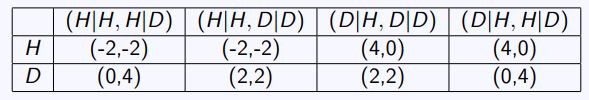
\includegraphics[width=0.7\linewidth]{images/DR6-Slide34}
\caption{}
\label{fig:DR6-Slide34}
\end{figure}

It can be seen that (H, [D|H, D|D]) is a (weak) Nash equilibrium
in this game, since neither player can increase their payoff by
unilaterally switching strategy.
%%- 34 / 61
%============================================%

%Subgame Perfect Equilibria in the Context of Matrix Games
However, the strategy [D|H, H|D] dominates the action
[D|H, D|D], since Player 2 always does as well by playing
[D|H, H|D] rather than [D|H, D|D] and does better when Player 1
plays D.
It can be shown that (H, [D|H, H|D]) is the only Nash equilibrium
left after the removal of dominated strategies.
%% 35 / 61
%============================================%
\subsection{Payoff Dominant Nash Equilibria}
\begin{itemize}
	\item A payoff vector (v1, v2) is said to Pareto dominate payoff vector
	(x1, x2) if v1 ≥ x1, v2 ≥ x2 and inequality is strict in at least one of
	the cases.
	\item	That is to say, Nash Equilibrium 1 of a game Pareto dominates
	Nash Equilibrium 2 if no player prefers Equilibrium 1 to Equilibrium
	2 and at least one player prefers Equilibrium 1.
	\item	A Nash equilibrium is payoff dominant if the value of the game
	corresponding to this equilibrium Pareto dominates all the values
	of the game corresponding to other equilibria.
\end{itemize}

%%- 36 / 61
%============================================%
%=================================================%
\subsection{Example}
Consider the following game
A B
A (4,4) (0,0)
B (0,0) (2,2)
Such a game is called a coordination game, as both players would
like to take the same action.
%%- 37 / 61
%============================================%
%=================================================%
\subsection{Example}
There are 3 Nash equilibria
1. (A, A) - Value (4,4).
2. (B, B) - Value (2,2).
3. (1/3A + 2/3B, 1/3A + 2/3B) - Value ( 4
3
,
4
3
).
The first equilibrium Pareto dominates the other two equilibria,
whilst the second equilibrium Pareto dominates the third.
(A, A) is the payoff dominant equilibrium.
%%- 38 / 61
%============================================%
\subsection{Risk Dominance}
\begin{itemize}
	\item Suppose there are pure Nash equilibria (A, C) and (B, D).
	\item The risk factor associated with strategy A, FA, is the probability
	with which Player 2 should play C (which is used at the Nash
	equilibrium where Player 1 plays A), in order to make Player 1
	indifferent between playing A or B.
	\item 	A high risk factor indicates that Player 1 must be relatively sure
	that Player 2 will play C for Player 1 to prefer A to B.
	\item 	Similarly, the risk factor associated with strategy B is the
	probability with which Player 2 should play D, in order to make
	Player 1 indifferent between playing A or B.
\end{itemize}

%%- 39 / 61
%============================================%
%%- \subsection{Risk Dominance}
\begin{itemize}
	\item The risk factors associated with C and D can be calculated in a
	similar way.
	\item The Nash equilibrium (A, C) risk dominates (B, D) if FA ≤ FB ,
	FC ≤ FD and there is strictly inequality in at least one case.
\end{itemize}

%%- 40 / 61
%============================================%
\subsection{Example}
Consider the following symmetric game
A B
A (4,4) (-1000,0)
B (0,-1000) (2,2)
It is clear that the equilibrium (A, A) payoff dominates the
equilibrium (B, B). However, there is a large risk associated with
playing action A (the possibility of obtaining a payoff of -1000).
%% 41 / 61
%=================================================%
%% \subsection{Example}
From the symmetry of the game, the risk factors of the two
strategies are the same for both players.
The risk factor associated with A is given by the solution of
4p − 1000(1 − p) = 0p + 2(1 − p) ⇒ p =
1002
1006
.
The risk factor associated with B is given by the solution to
2p + 0(1 − p) = −1000p + 4(1 − p) ⇒ p =
4
1006
.
It follows that B risk dominates A.
%% 42 / 61
%============================================%
\subsection{Conclusion}
\begin{itemize}
	\item If an equilibrium both payoff and risk dominates another, it seems
	clear that this should be the one chosen.
	\item In other cases, it is not clear what equilibrium should be played.
	\item The concept of risk domination is important in evolutionary game
	theory (see later).
\end{itemize}

%%- 43 / 61
%============================================%
%=================================================%
\subsection{3.7 2-Player Games with a Continuum of Strategies and
Simultaneous Moves}
\begin{itemize}
	\item Assume that Player i chooses an action from a finite interval Si
	.
\item The payoff to Player i when Player 1 takes action x1 and Player 2
	takes action x2 is given by Ri(x1, x2).
\item It is assumed that the payoff functions are differentiable.
\end{itemize}

%%- 44 / 61
%============================================%
\subsection{The Symmetric Cournot Game}
\begin{itemize}
\item Assume that two firms produce an identical good. Firm i produces
xi units per time interval.
\item The price of the good is determined by total supply and all
production is sold at this ”clearing price”. It is assumed that
p = A − B[x1 + x2], (A, B > 0).
\item The costs of producing x units of the good are assumed to be
C + Dx for both firms.
\item The payoff of a firm is taken to be the profit obtained (revenue
minus costs). Revenue is simply production times price.
\end{itemize}

%% 45 / 61
%============================================%
\subsection{The Symmetric Cournot Game}
The payoff obtained by Firm 1 is given by
\[R1(x1, x2) = px1 − C − Dx1 = (A − D)x1 − Bx2
1 − Bx1x2 − C.\]
By symmetry, the payoff obtained by Player 2 is
\[R2(x1, x2) = px2 − C − Dx2 = (A − D)x2 − Bx2
2 − Bx1x2 − C.\]
It should be noted that it clearly does not pay firms to produce
more than the amount xmax that guarantees that the price is equal
to the unit (marginal) cost of production. Since xmax is finite, we
may assume that firms choose their strategy (production level)
from a finite interval.
%% 46 / 61
%============================================%
\subsection{Best Response Functions}
Given the output of the opponent, we can calculate the optimal
response of a player using calculus.
Let B1(x2) denote the best response of Player 1 to x2.
Let B2(x1) denote the best response of Player 2 to x1.
47 / 61
Nash Equilibria in Games with a Continuum of Strategies
and Simultaneous Actions
At a Nash equilibrium (x
∗
1
, x
∗
2
), we have
x
∗
1 = B1(x
∗
2
); x
∗
2 = B2(x
∗
1
).
Thus, at a Nash equilibrium Player 1 plays her best response to
Player 2’s strategy and vice versa.
%%- 48 / 61
%============================================%
\subsection{The Cournot Game}
Suppose A = 3, B =
1
1000 , C = 100 and D = 1.
We have
R1(x1, x2) = 2x1 −
x
2
1
1000
−
x1x2
1000
− 100.
In order order to derive the best response of Player 1 to Player 2’s
action, we differentiate Player 1’s payoff function with respect to
x1, his action.
%%- 49 / 61
%============================================%
\subsection{The Cournot Game}
We have
∂R1(x1, x2)
∂x1
= 2 −
2x1 + x2
1000
.
It should be noted that this derivative is decreasing in x1, hence
any stationary point must be a maximum.
The optimal response is given by
2 −
2x1 + x2
1000
= 0 ⇒ x1 = 1000 −
x2
2
.
Thus B1(x2) = 1000 −
x2
2
.
%% 50 / 61
%============================================%
\subsection{The Cournot Game}
It should be noted that this solution is valid as long as x2 ≤ 2000
(production cannot be negative).
If x2 > 2000, then ∂R1(x1,x2)
∂x1
is negative for all non-negative values
of x1.
In this case the best response is not to produce anything.
%%- 51 / 61
%============================================%
\subsection{The Cournot Game}
By symmetry the best response of Player 2 is given by
B2(x1) = max{0, 1000 −
x1
2
}.
We look for an equilibrium at which both firms are producing. In
this case
x
∗
1 = 1000 −
x
∗
2
2
; x
∗
2 = 1000 −
x
∗
1
2
.
It follows that at Nash equilibrium both firms must produce 2000
3
units.
Intuitively, from the form of the game both firms should produce
the same amount.
%%- 52 / 61
%=================================================%
\subsection{The Cournot Game}
The value of the game can be found by substituting these values
into the payoff functions.
R1(x
∗
1
, x
∗
2
) = R2(x
∗
1
, x
∗
2
) = 2 ×
2000
3
− 2 ×
1000
9
− 100 ≈ 344.
The equilibrium price is 3 − 2 ×
2
3 =
5
3
.
%%- 53 / 61
%============================================%
\subsection{The Cournot Game}
\begin{itemize}
	\item There cannot be an equilibrium at which one of the firms does not
	produce. The argument is as follows.
	\item If one firm does not produce, then the optimal response to this is
	to produce 1000 units.
	\item (0,1000) cannot be a Nash equilibrium, since the best response of
	Firm 1 to x2 = 1000 is to choose x1 = 500.
\end{itemize}

%%- 54 / 61
%============================================%
\section{The Stackelberg Model}
This is identical to the Cournot model, except that it is assumed
that one of the firms is a market leader and chooses its production
level before the second firm chooses.
The second firm observes the production level of the first.
%%- 55 / 61
%============================================%
\subsection{Games with a Continuum of Strategies and Sequential Moves}
Suppose Player 2 moves after Player 1 and observes the action
taken by Player 1. The equilibrium is derived by recursion.
Player 2 should choose the optimum action given the action of
Player 1.
Hence, we first need to solve
∂R2(x1, x2)
∂x2
= 0.
This gives the optimal response of Player 2 as a function of the
strategy of Player 1, x2 = B2(x1).
56 / 61
%============================================%
\subsection{Games with a Continuum of Strategies and Sequential}
Moves
We now calculate the optimal strategy of the first player to move.
If Player 1 plays x1, Player 1 responds by playing B2(x1). Hence,
we can express the payoff of Player 1 as a function simply of x1,
i.e. R1(x1, B2(x1)).
In order to find the optimal action of Player 1, we differentiate this
function with respect to x1.
Having calculated the optimal value of x1, we can derive x2.
57 / 61
%============================================%
\subsection{Example}
Derive the equilibrium of the Stackelberg version of the previous
example.
We have
R2(x1, x2)=2x2 −
x
2
2
1000
−
x1x2
1000
− 100.
∂R2(x1, x2)
∂x2
=2 −
x2
500
−
x1
1000
.
58 / 61
%============================================%
\subsection{Example}
It follows that the best response of Player 2 is given by
2 −
x2
500
−
x1
1000
= 0 ⇒ x2 = 1000 −
x1
2
.
Hence,
R1(x1, B2(x1))=R1(x1, 1000 −
x1
2
)
=2x1 −
x
2
1
1000
−
x1(1000 − x1/2)
1000
− 100
=x1 −
x
2
1
2000
− 100.

\begin{figure}[h!]
\centering
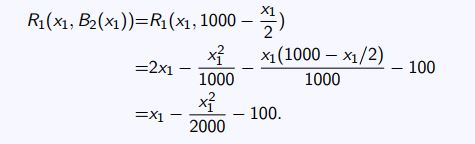
\includegraphics[width=0.7\linewidth]{images/DR6-Slide59}
\caption{}
\label{fig:DR6-Slide59}
\end{figure}

%%- 59 / 61
%============================================%
\subsection{Example}
Differentiating
\[∂R1(x1, B2(x1))
∂x1
= 1 −
x1
1000
.\]
It follows that Firm 1 maximises its profit by producing 1000 units.
The best response of Firm 2 is B2(x1) = 1000 −
x1
2 = 500 units.
The Stackelberg equilibrium is (1000, 500). Hence, the leader
produces more than at the Cournot equilibrium and the follower
produces less.
Total production is greater than at the Cournot equilibrium, i.e.
the equilibrium price is lower.
%% 60 / 61
%============================================%
\subsection{Example}
The profit of Firm 1 at this equilibrium is
\[R1(1000, 500) = 2 × 1000 − 1000 − 500 − 100 = 400.\]
The profit of Firm 2 at this equilibrium
\[R2(1000, 500) = 2 × 500 − 250 − 500 − 100 = 150.\]
It is clear that Firm 1 gains by being the leader. Firm 2 loses. The
sum of profits is lower than at the Cournot equilibrium.
This seems somewhat counter-intuitive, as the market would seem
to be more competitive under the Cournot model.
%% 61 / 61


\end{document}